\chapter{Developer Guidelines}
\label{DeveloperGuidelines}

CrypTool 2.0 uses state-of-the-art technologies like .NET 3.5 and WPF. In order to make your first steps towards developing something in the context of this project, a few things need to be considered. First of all, please follow the instructions in this document so that you do not get stuck. If you encouter a problem or error that is not described here, please let us know so we can add the appropriate information to this guide.

In the following sections we will describe all steps necessary in order to compile CrypTool 2.0 on your own. This is always the first thing you need to do before you can begin developing your own plugins and extensions. The basic steps are:
\begin{itemize}
	\item Getting all prerequisites and installing them
	\item Accessing and downloading the source code with SVN
	\item Compiling the current source code for the first time
\end{itemize}

\section{Prerequisites}
\label{Prerequisites}

Since CrypTool 2.0 is based on Microsoft .NET 3.5, you will need a Microsoft Windows environment. (Currently no plans exist for porting this project to mono or to other platforms.) We have successfully tested with \textbf{Windows XP}, \textbf{Windows Vista} and \textbf{Windows 7}.

Since you are reading the developer guidelines, you probably want to develop something. Hence, you will need a development environment. In order to compile our sources you need \textbf{Microsoft Visual Studio 2008 Professional}. Please always install the latest service packs for Visual Studio. Unfortunately, our sources do not work (smoothly) with the freely available Visual Studio Express (C\#) versions. This is due to the fact that CrypWin uses a commercial component and is therefore distributed only as binary, and the current version of C\# Express cannot handle a binary as a start project, which makes debugging cumbersome. This will be resolved later in 2010 when the project is moved to Visual Studio 2010.

Usually the installation of Visual Studio also installs the .NET framework. In order to run or compile our source code you will need (at the time of writing) at least \textbf{Microsoft .NET 3.5 with Service Pack 1 (SP1)}. You can get this for free from Microsoft's \href{http://download.microsoft.com/download/2/0/e/20e90413-712f-438c-988e-fdaa79a8ac3d/dotnetfx35.exe}{webpage}. Once that has been installed, your development environment should be ready for our source code.

\section{Accessing Subversion (SVN)}
\label{AccessingSubversion}

Now you will need a way of accessing and downloading the source code. In the CrypTool 2.0 project we use Subversion (SVN) for version control, and hence you need an \textbf{SVN client}, e.g.\ \textbf{TortoiseSVN} or the \textbf{svn commandline from cygwin}. It does not matter which client you use, but if you have never worked with SVN before, we suggest using \href{http://www.tortoisesvn.net/}{TortoiseSVN}, since it offers a nice Windows Explorer integration of SVN.
\clearpage

\subsection*{The CrypTool2 SVN URL}
\label{TheCrypTool2SVNURL}

Our code repository is accessable at the following URL:

\url{https://www.cryptool.org/svn/CrypTool2/}

To access the repository, you must provide a username and password. If you are a guest and just want to download our source code, you can use ``anonymous" as the username and an empty password. If you are a registered developer, just use your provided username and password (which should be the same as for the wiki).

\subsection*{Accessing the repository with TortoiseSVN}
\label{AccessingTheRepositoryWithTortoiseSVN}

As mentioned above, in order to access the SVN repository one of the best options is \href{http://www.tortoisesvn.net/}{TortoiseSVN}. We will describe here how to use the basics of the program, although you should be able to use any SVN client in a similar fashion.

\begin{figure}[h!]
	\centering
		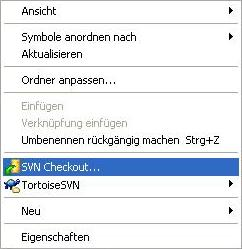
\includegraphics[width=0.40\textwidth]{figures/tortoise_svn_checkout.jpg}
	\caption{Selecting ``SVN Checkout" from the context menu after installing TortoiseSVN.}
	\label{fig:tortoise_svn_checkout}
\end{figure}

First install TortoiseSVN (which unfortunately requires you to reboot your computer) and then create a directory (for instance ``CrypTool2") for storing the local working files somewhere on your computer. Right-click on this directory and select ``SVN Checkout" from the context menu. A window will appear in which you will be asked for the URL of the repository; use the address given above, as seen in Figure \ref{fig:tortoise_svn_checkout2}. The ``Checkout directory" should already be filled in correctly with your new folder. Then just hit ``OK", accept the certificate (if necessary), and enter your login information as described above. Mark the checkbox for saving your credentials if you don't want to enter them every time you work with the repository. Then hit ``OK", and now the whole CrypTool2 repository should be checked out into your chosen directory.
\clearpage

\begin{figure}[h!]
	\centering
		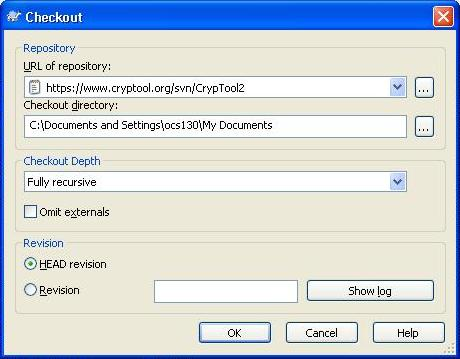
\includegraphics[width=0.60\textwidth]{figures/tortoise_svn_checkout2.jpg}
	\caption{Checking out the CrypTool2 repository.}
	\label{fig:tortoise_svn_checkout2}
\end{figure}

Later on, if changes have been made in the repository and you want to update your working copy, you can do this by right-clicking on any directory within the working files and choosing ``SVN Update" from the context menu. You should do this often to maintain a current version of the files.

A TortoiseSVN tutorial can be found \href{http://www.mind.ilstu.edu/research/robots/iris4/developers/svntutorial}{here}.

\subsection*{Committing your changes}
\label{CommitingYourChanges}

If you are a registered developer, you can commit your file changes to the public CrypTool2 repository. Right-click on the directory within the working files that contains your changes and select ``SVN Commit" from the context menu to upload your changes. Please always provide \textit{meaningful descriptions} of your updates. You should commit your sources to our SVN repository as often as you can to ensure your interoperability with the rest of the project, but only commit code that successfully compiles and runs!

\begin{figure}[h!]
	\centering
		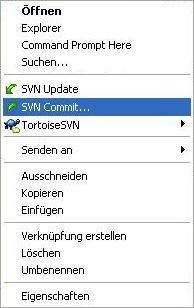
\includegraphics[width=0.40\textwidth]{figures/tortoise_svn_commit.jpg}
	\caption{Selecting ``SVN Commit" from the context menu.}
	\label{fig:tortoise_svn_commit}
\end{figure}

You can use command words in the SVN comment to link your changes to a particular ticket. The command syntax is as follows:

\begin{center}
\fbox{\parbox{15cm}
{\tt
command \#1\newline
command \#1, \#2\newline
command \#1 \& \#2\newline
command \#1 and \#2
}}
\end{center}

You can have more than one command in a message. The following commands are supported. There is more than one spelling for each command, to make this as user-friendly as possible.

\begin{center}
\fbox{\parbox{15cm}
{\tt
closes, fixes:\newline
  The specified issue numbers are closed with the contents of this
  commit message being added to it.

references, refs, addresses, re:\newline
  The specified issue numbers are left in their current status, but
  the contents of this commit message are added to their notes.
}}
\end{center}

A fairly complicated example of what you can do is with a commit message of:

\begin{center}
\fbox{\parbox{15cm}
{\tt
Changed blah and foo to do this or that.\ Fixes \#10 and \#12, and refs \#12.
}}
\end{center}

This will close \#10 and \#12, and add a note to \#12.

\subsection*{Ignore patterns}
\label{IgnorePatterns}

Please only check in proper source code by using the following \textbf{ignore patterns}:

\begin{center}
\textit{obj bin debug release *.pdb *.suo *.exe *.dll *.aux *.dvi *.log *.bak *.bbl *.blg *.user}
\end{center}

This basically means that you should never check in compiled and automatically generated files. For example, please do not check in the entire \textit{bin/} and \textit{obj/} directories that Visual Studio generates. Note that the server will reject your commits if you try to do so. If you want to submit a component (binary file) despite the ignore patterns you can still add \textit{*.dll} files by using the context menu and adding the file explicitly - but please be absolutely sure that you know what you are doing. Additionally, you need to provide an explicit list of file and directory names which should override the ignore pattern. For example, if you want to check in a file named someLib.dll, you must write a comment which looks like this:

\begin{center}
\fbox{\parbox{15cm}
{\tt
The lib is required by all developers, so I am adding it explicitly to the repository.

override-bad-extension:\ someLib.dll
}}
\end{center}

Please note that any text after the colon and the whitespace will be treated as the file name. Therefore, do not use quotation marks and do not write any text after the file name.
\clearpage

\section{Compiling the sources}
\label{CompilingTheSources}

By this point you should have checked out a copy of the entire CrypTool repository. Compiling is pretty easy; just go to the \textit{trunk/} directory and open the \textbf{\textit{CrypTool 2.0.sln}} Visual Studio solution. The Visual Studio IDE should open with all the working plugins components nicely arranged. In case you are now starting Visual Studio for the first time, you will have to choose your settings. Just select either ``most common" or ``C\#" --- you can change this at any time later. On the right side is the project explorer, where you can see all the subprojects included in the solution. Look for the project \textbf{\textit{CrypWin.exe}} there. Once you have found it, right-click on it and select ``Set as StartUp-Project" from the context menu. Next, go to the menu bar and select ``Build" $\rightarrow$ ``Build Solution".

Then go to ``Debug" and select ``Start Debugging". CrypTool 2.0 should now start for the first time with your own compiled code. Presumably you have not changed anything yet, but you now have your own build of all the components (with the exception of CrypWin and AnotherEditor, since they are available only as binaries). If the program does not compile or start correctly, please consult our \href{https://www.cryptool.org/trac/CrypTool2/wiki/FAQ}{FAQ} and let us know if you found a bug.

If you are a \textbf{core developer}, hence somebody who can also compile CryWin and AnotherEditor, you should use the \textbf{\textit{CrypTool 2.0.sln}} solution from the \textit{trunk/CoreDeveloper/} directory (which will \textit{not} be visible to you if you are not a core developer). As a core developer, be aware that when you compile, you \textbf{change the \textit{CryWin.exe}} that is visible to everybody else. Thus, when doing a check-in, please make sure you \textit{really} want to check in a new binary. Core developers can also build a new setup and publish it as beta release on the website. This process is explained in the wiki at \url{https://www.cryptool.org/trac/CrypTool2/wiki/BuildSetup}.